\documentclass{standalone}
\usepackage{tikz}
\usepackage{ctex,siunitx}
\usepackage{tkz-euclide}
\usepackage{amsmath}
\usetikzlibrary{patterns, calc}
\usetikzlibrary {decorations.pathmorphing, decorations.pathreplacing, decorations.shapes,}
\begin{document}
\small
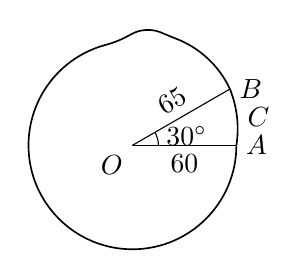
\begin{tikzpicture}[>=latex,scale=0.22]
  \draw [semithick,domain=0:30,samples=200] plot (\x:{6+\x/60})coordinate(B);
  \draw[semithick](6,0)arc(360:105:6)arc(-75:-60:6)arc(120:70:2)coordinate(C);
  \draw[semithick](B)arc(25:70:5.7)--(C);
  \draw(0,0)--(30:6.5)node[midway,sloped,above]{65};
  \draw(0,0)--(6,0)node[midway,below]{60};
  \draw(1.5,0)arc(0:30:1.5)node[pos=0.7,right]{\ang{30}};
  \node at (0,0) [below left]{$O$};
  \node at (6,0) [right]{$A$};
  \node at (30:6.5) [right]{$B$};
  \node at (15:6.3) [right]{$C$};
\end{tikzpicture}
\end{document}